    \documentclass[12pt, twoside, notitlepage, twocolumn]{article}
    \setlength{\columnsep}{0.5cm}
    \usepackage[a4paper, left=0.5cm,right=0.5cm,top=0cm,bottom=0.5cm]{geometry}
    \usepackage{amsmath,bm}
    \usepackage{sectsty}
    \usepackage{graphicx}
    \usepackage{tabularx}
    \usepackage{hyperref}
    \sectionfont{\fontsize{12}{12}\selectfont}
    \setlength{\parindent}{0pt}

% Document begins
    \begin{document}
        \twocolumn[\begin{@twocolumnfalse}
            \begin{flushleft}
                \textbf{Measurement of $\bm{CP}$ Violation in $\bm{B^{\pm}\rightarrow\pi^{\pm}\pi^{+}\pi^{-}}$ 
                Decay Channal at Large Hadron Collider\newline}
                Qichen Dong, Harriet Watson\newline
                School of Physics and Astronomy, University of Manchester, Manchester, M13 9PL.
                
            \end{flushleft}
            \textbf{Abstract:} A set of selected $p p$ collision data samples which were collected by 
                LHCb\cite{1748-0221-3-08-S08005} in 2011 are studied.
                Contained $B^{\pm}\rightarrow\pi^{\pm}\pi^{+}\pi^{-}$ decays in magnet ``up'' and ``down'' 
                polarities are constructed. Global $CP$ asymmetry in this channel is measured to be 
                $A_{CP}=0.126\pm0.023\pm0.026$,
                in which the first and second uncertainties are statistical and systematic respectively. 
                Larger asymmetry in local area of phase space is also observed.\newline\hbox{}
        \end{@twocolumnfalse}]

        \section{Introduction}
        The Standard Model (SM)\cite{1412.4094} of particle physics, which developed in early 1970s, has been successfully 
        explaining almost all experiment results and made precise predictions.
        Although the SM has been considered as the best theory describing fundamental particles and their interaction, phenomena such as large scale of matter antimatter 
        asymmetry in the universe are not fully explained. Matter antimatter asymmetry is described by Charge
        Parity (CP) invariance violation in the SM, but the effect is too small to explain observed magnitude.
        Therefore, additional sources of CP violation above SM
        may contributes to the exceeding magnitude of asymmetry. Charmless B meson to 3 hadrons decay is observed 
        to have the largest CP violation. Measuring CP violation provides evidence of physics beyond The SM.
        \section{Candidates Selection}
        The LHCb\cite{1748-0221-3-08-S08005} detector is designed for studying particles containing $b$ and $c$ quark.
        Analysed data was preselected by hardware and software trigger from approximately $10^{14}$ $pp$ collision
        events with centre-of-mass energy of 7 TeV. Most important pre-selection cuts are listed in the labscript\cite{Labsc}.
        Information from the particle identification system\cite{1211.6759} are used to separate
        $B^{\pm}\rightarrow\pi^{\pm}\pi^{+}\pi^{-}$ events. Apart from rejecting muon, the probability of each 
        particle to be a pion is required to be larger than 0.794 to make sure 50 per cent $B$ candidates have final states of 3 pion.
        CP Asymmetry introduced by charmed decay of B mesons are removed by rejecting $D^0$ 
        resonance by excluding $\pm 50MeV$ region of $D^0$ meson mass in two body invariant mass $M_{\pi^+\pi^-}$ spectrum. 
        \section{Global Asymmetry}
        Raw asymmetry of $B^{\pm}\rightarrow\pi^{\pm}\pi^{+}\pi^{-}$ mode is defined as $A_{raw} = \epsilon^--\epsilon^+$, 
        where $\epsilon^\pm = \frac{N_{B^\pm}}{N_{B^+}+N_{B^-}}$ is efficiency. $N_{B^\pm}$ is estimated by fitting $B$ 
        meson invariant mass spectra and integrating contribution of signal models. Cruijff function with zero right radiative 
        tail was chosen to be signal model, the mean, width and left tail parameters were left free. We described the combinatorial 
        background by an exponential function, all of its parameters were left to be fitted. Backgrounds caused by four-body-decay 
        were parametrized by gaussian, whose peak positions were fixed to 5134 MeV for $B^+$ and 5040 MeV for $B^-$ by optimizing 
        deduced $\chi^2$ of fitting, We also tried to introduce a small peak centred in 5215 MeV to describe 
        $B^{\pm}\rightarrow K^{\pm}\pi^{+}\pi^{-}$ in which one Kaon was misidentified, however, contribution of it is negligible 
        with rather strict selection criteria we implemented. The invariant mass contribution and fitting results are shown in figure 1.
        \begin{figure}[!hb]
            \begin{centering}
            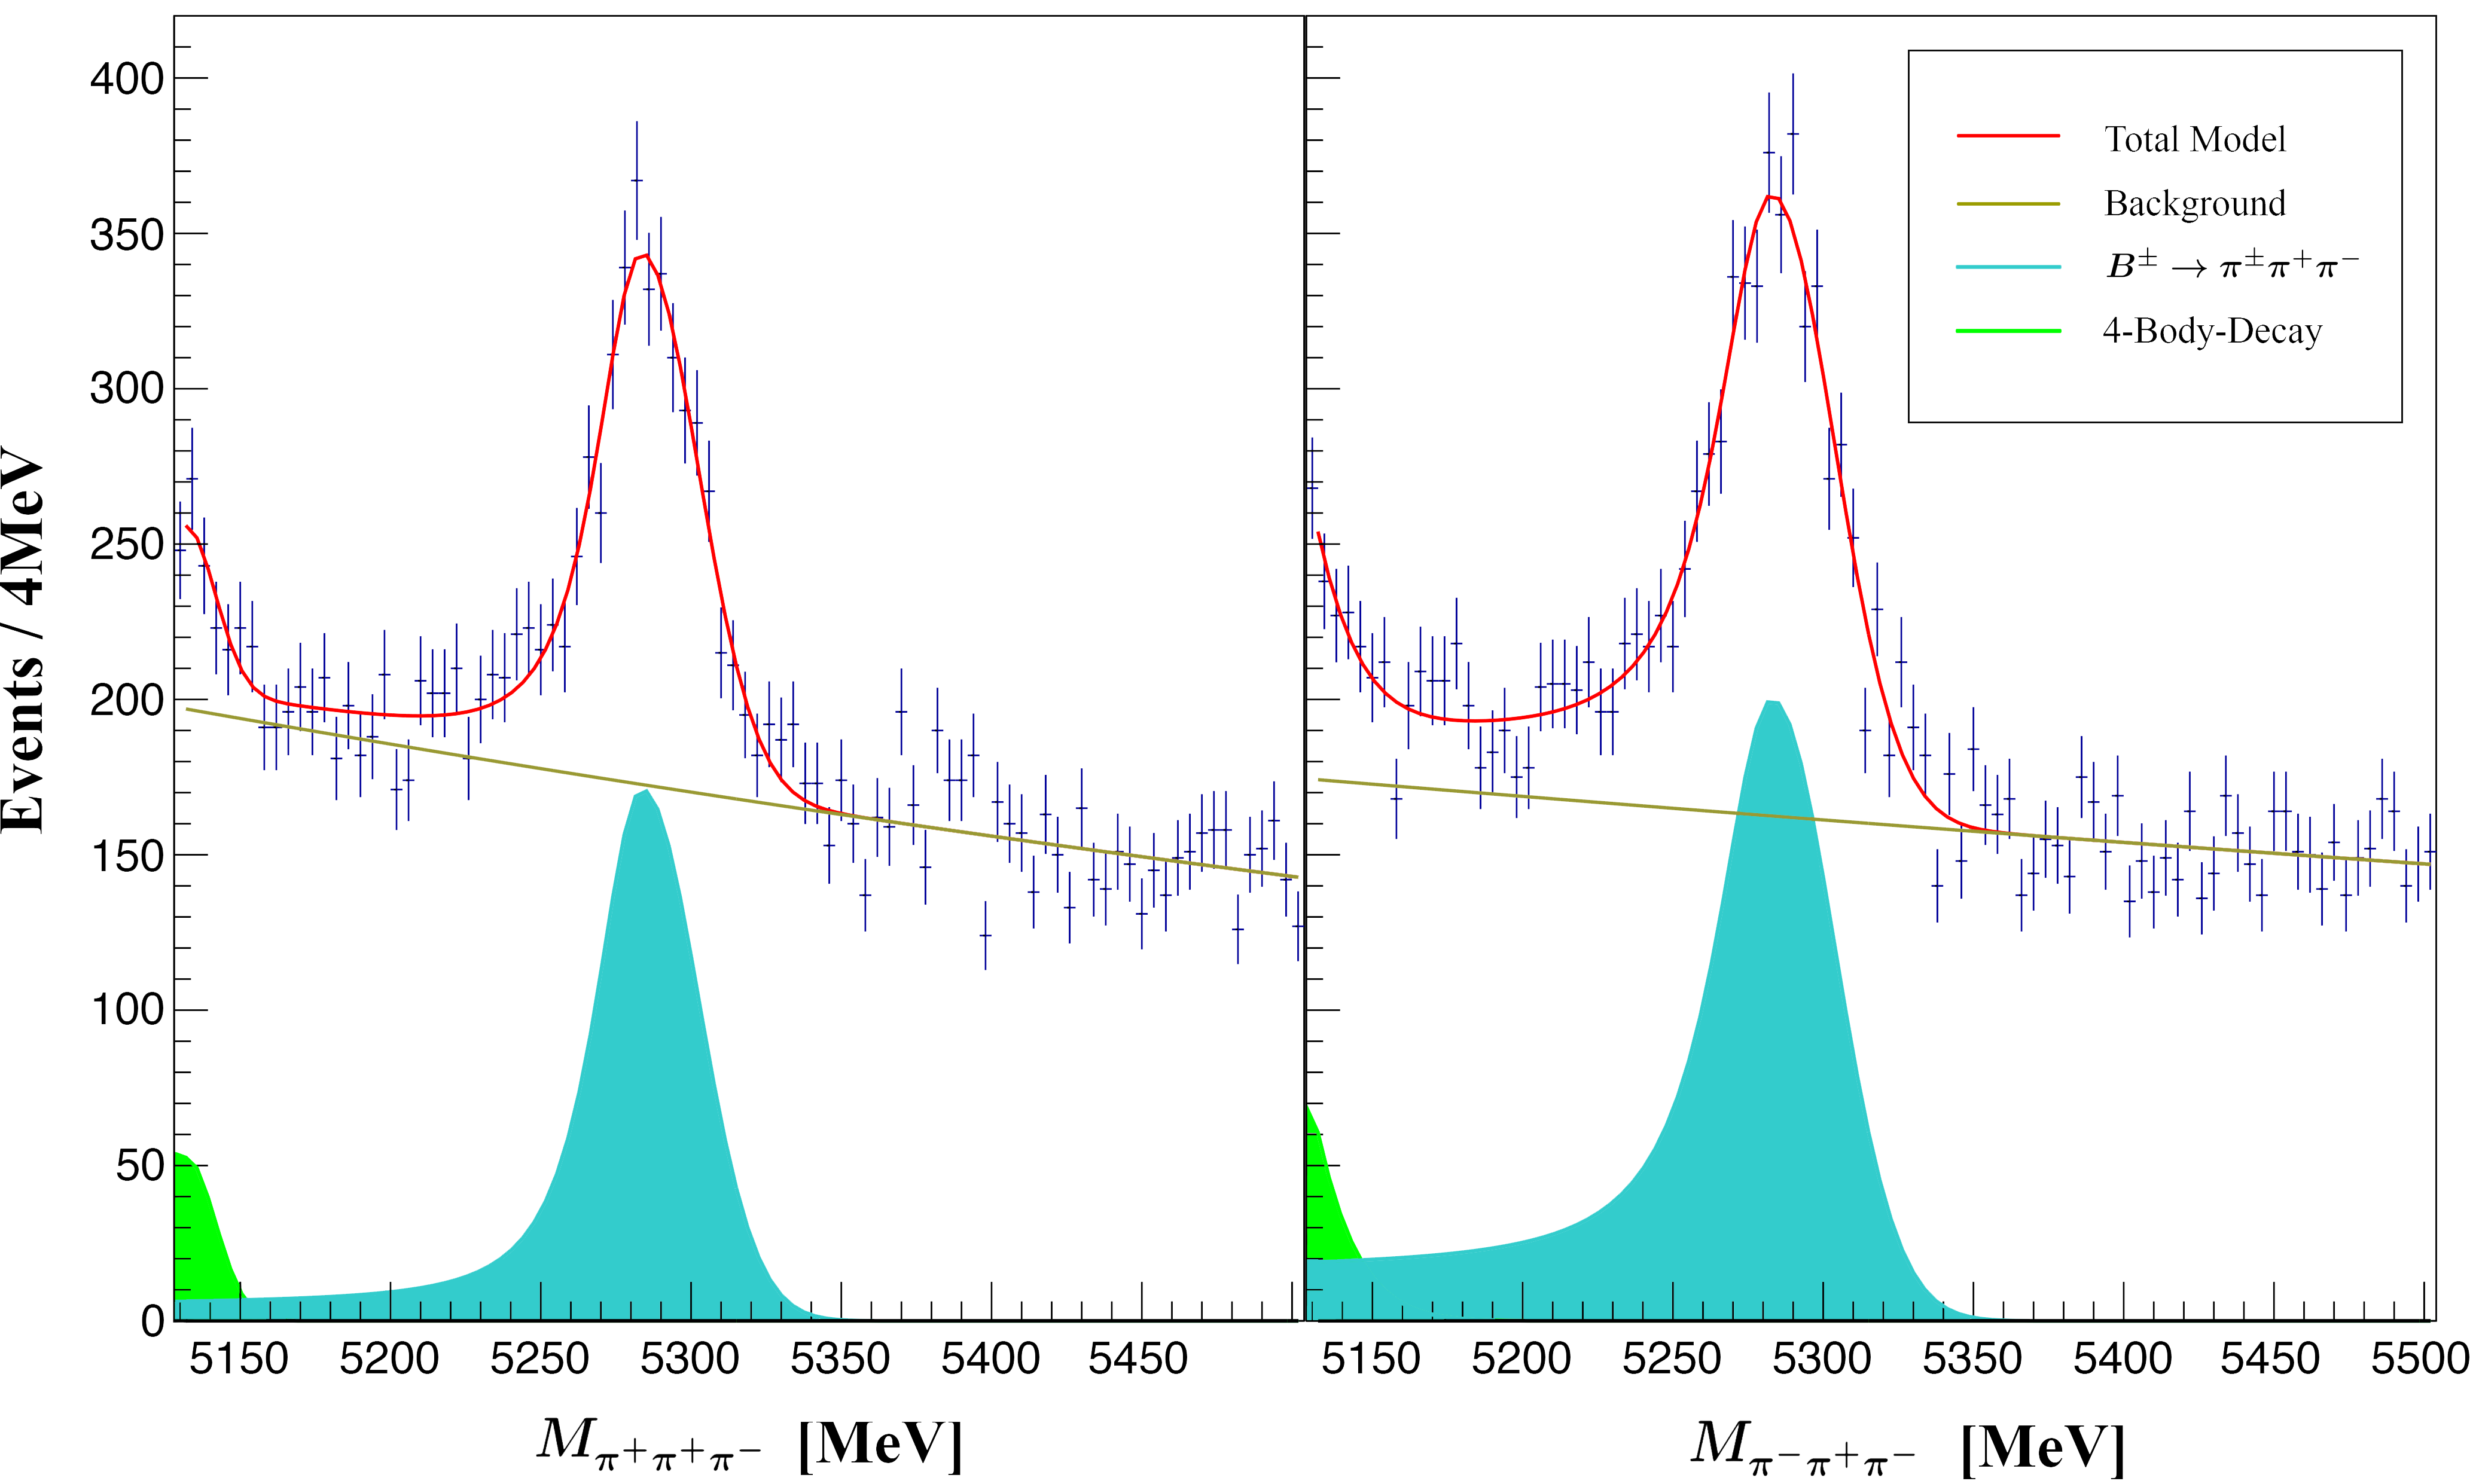
\includegraphics[scale=0.276]{GA.png}
            \caption{Invariant mass spectra and fitting results. \newline Left panel is $B^+$ and Right panel is $B^-$}
            \end{centering}
            \label{fig:label1}
        \end{figure}
        Integration of signal model gives $N_{B^+} = 2251 \pm 81$ and $N_{B^-} = 2789 \pm 82$. Raw CP asymmetry yields $A_{raw}=0.107 
        \pm 0.023 (statistical)$. Since detector efficiencies for $B^+$ and $B^-$ are not equal in different magnet polarities, a detector 
        polarity correction is made based on $\epsilon^\pm_{up}$ and $\epsilon^\pm_{down}$ in two subsets of data, defined as 
        $A_{cor}=\epsilon_{cor}^--\epsilon_{cor}^+$, where $\epsilon_{cor}^\pm = (\epsilon^\pm_{up}+\epsilon^\pm_{down})/2$.
        $A_{CP}$ is calculated by excluding B-meson production asymmetry $A_P = -0.004\pm0.004$\cite{1310.4740} from $A_{cor}$, which 
        yields $A_{CP} = A_{cor} - A_P = 0.126 \pm 0.023$, Uncertainty above is statistical only, estimated by integrating 
        fitting-error within 3-sigma width around signal mean. 4 aspects of sources of systematic uncertainties were studied. Uncertainty 
        introduced by polarity correction is significantly larger than other sources, estimated by $\pm(A_{raw}-A_{cor})$. Method used in 
        calculating error of chosen signal model is comparing $A_{raw}$ given by ``similar-good-fit'' Cruijff function and double 
        gaussian signal model, defined as $\pm(A_{raw}^{Cruijff}-A_{raw}^{Gaussian})$. This two function give deduced 
        $\chi^2_+=1.109,\ \chi^2_-=1.065$ and $\chi^2_+=1.162,\ \chi^2_-=1.118$ respectively. Lorentz function was not included since it gives relatively 
        higher deduced $\chi^2$. By shifting the position of 4-body gaussian function, we estimated uncertainty of partially reconstructed 
        4-body-decay. However, its magnitude is around $10^{-5}$, which is negligible. B meson production uncertainty was considered as 
        systematic error. Total \newpage\newgeometry{left=0.5cm,right=0.5cm,top=0.3cm,bottom=0.5cm} systematic uncertainty is calculated 
        by sum in quadrature of each contribution, main systemetic uncertainties are listed in Table 1.
        \begin{table}[ht]
            \centering
            \caption{Main systematic Uncertainties}
            \begin{tabularx}{9.73cm}{lXr}
            \hline
            Source & & Uncertainty \\
            \hline
            Polarity Correction  & & 0.023 \\
            Signal Function  & & 0.011 \\
            4-body Backgrounds & & 0.000 \\
            B Meson Production & & 0.004 \\
            \hline
            Total & & 0.026 \\
            \hline
            \end{tabularx}
        \end{table}
        \newline In summary, inclusive CP asymmetry is measured to be $A_{CP} = 0.126\pm0.023(statistical)\pm0.026(systematical)$
        total uncertainty is calculated by $\pm \sqrt{0.023^2+0.026^2}=\pm 0.035$, significance yeilds $3.63\sigma$.
        \section{Local Asymmetry}
        \begin{figure}[b]
            \begin{centering}
            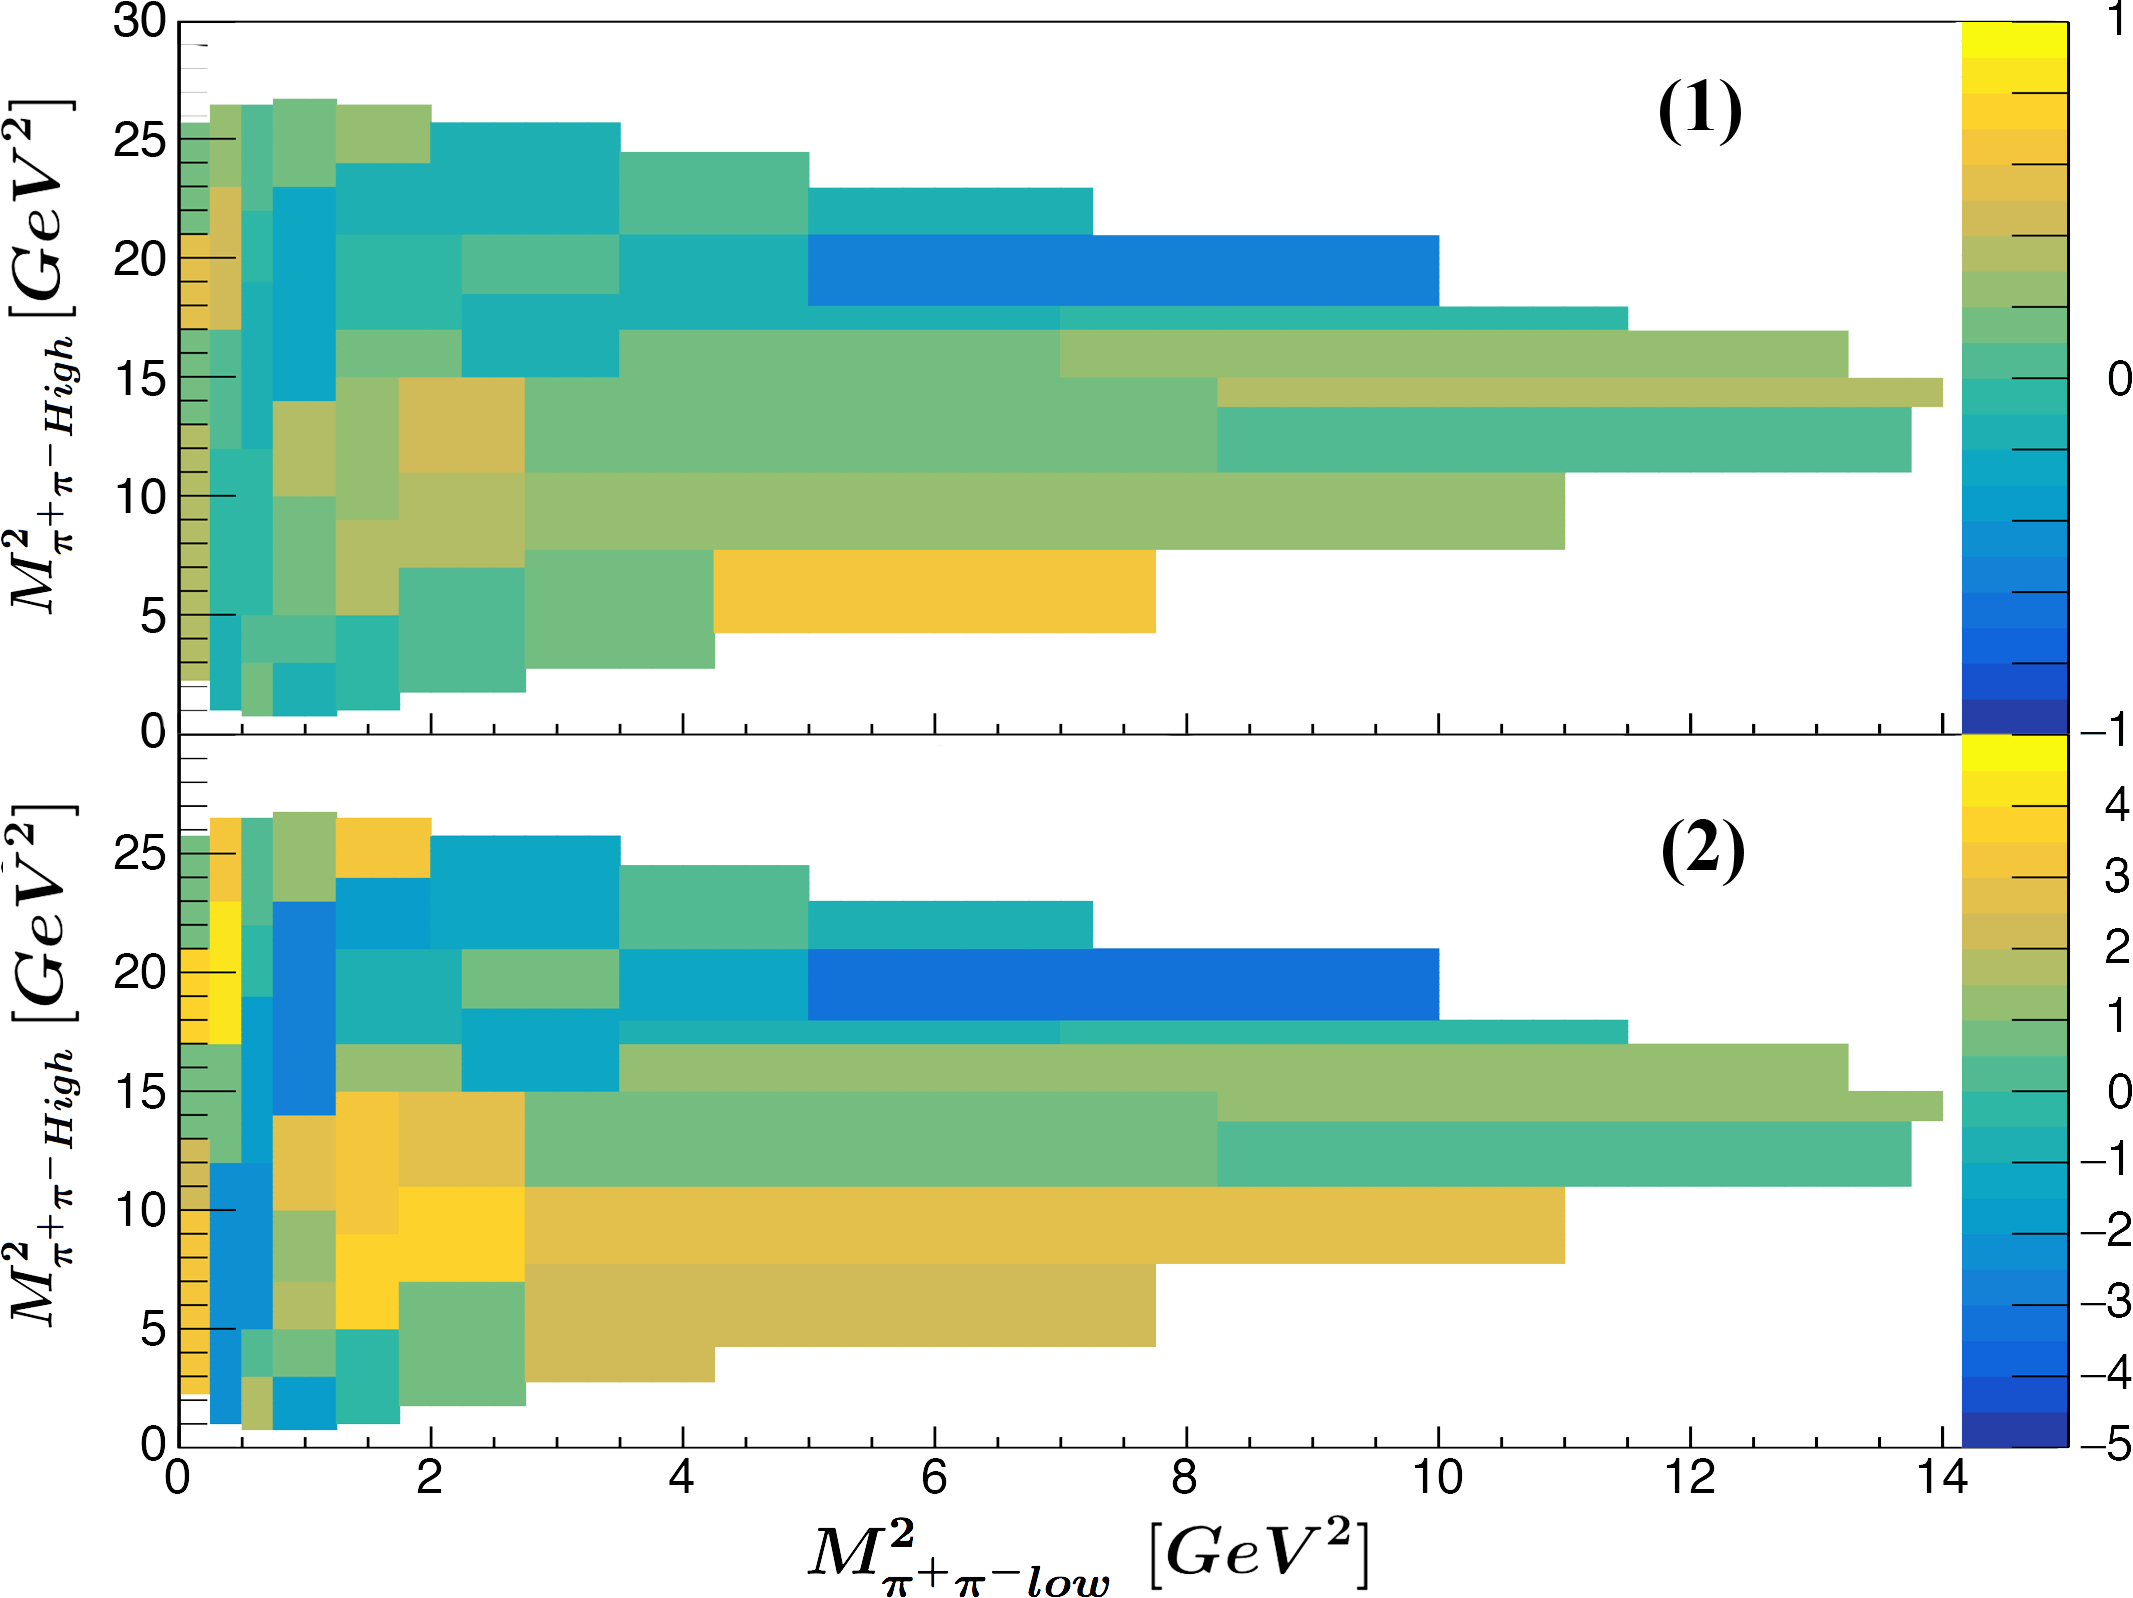
\includegraphics[scale=0.53]{LocalAS.png}
            \caption{(1) Asymmetries distributed in phase space.\newline (2) Significance in local phase space area.}
            \end{centering}
            \label{fig:label2}
        \end{figure}
        In order to investigate the distribution of CP violation, we studied local asymmetries in 
        2-body mass $M_{high\ \pi^+\pi^-}^2$ and $M_{low\ \pi^+\pi^-}^2$ phase space. Candidates whose
        mass are within $2\sigma$ width of signal model on 3-body mass spectrum are selected to be 
        combined signal. Background are defined as the average candidates in a 7 times wider region on 
        the higher-mass side adjoin the signal region. The background distribution was rescaled linearly 
        to match the distribution of signal in Dalitz plot. We set different bin size across the phase space
        to make sure every bins have approximately equal number of events. Asymmetries in $i^{th}$ 
        bin was calculated by $A_i=\frac{N^-_i-N^+_i}{N^+_i-N^+_i}$, corresponding error is statistical only.
        Asymmetry and significance are shown in Figure 2.
        $Area\ 1,\ [M^2_{low} \in (0,0.5),\ M^2_{high}\in(17,24)]$ and 
        $Area\ 2,\ [M^2_{low} \in (1,3),\ M^2_{high}\in(5,15)]$ have relatively high asymmetries and significances, 
        while $Area\ 3,\ [M^2_{low} \in (5,10),\ M^2_{high}\in(18,21)]$ has high significance but negative 
        asymmetry. Same methods used in measuring global CP asymmetry were used in these areas to evaluate 
        the original results. Results in local areas are shown in Figure 3.
        \begin{figure}[!ht]
            \begin{centering}
            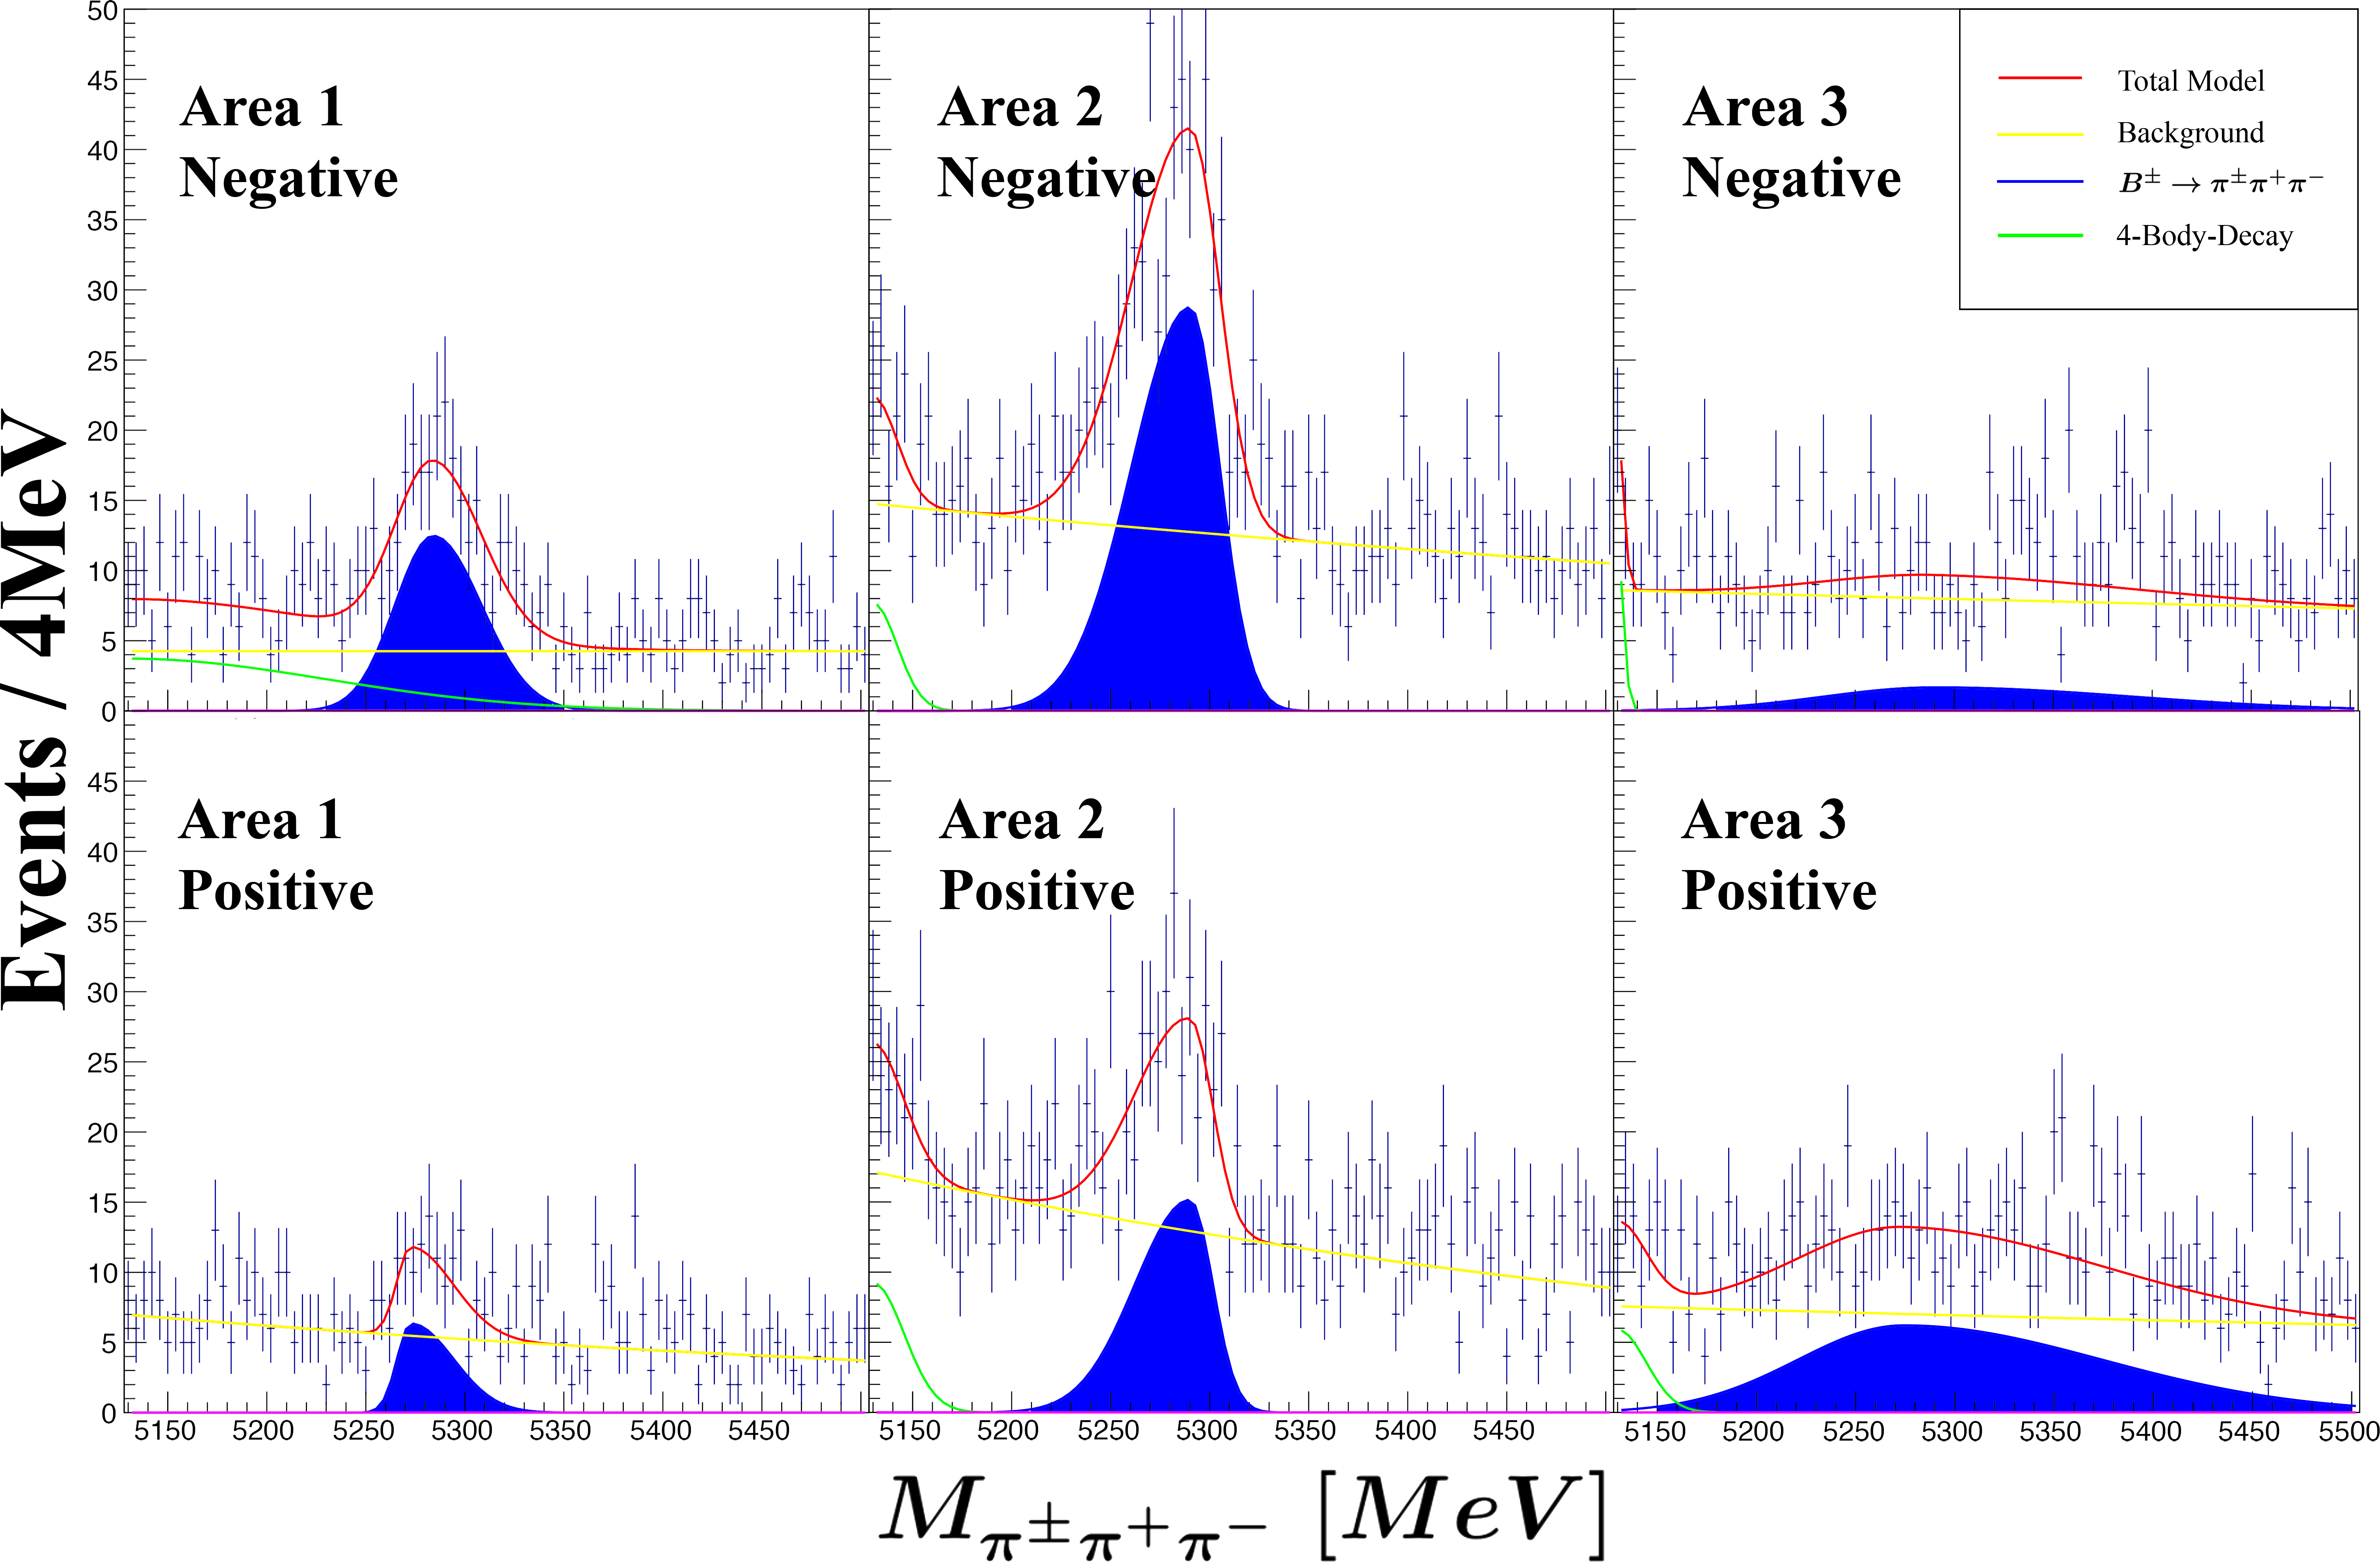
\includegraphics[scale=0.185]{ZoomFinal.png}
            \caption{Invariant mass spectrum and fitting results in local areas}
            \end{centering}
            \label{fig:label3}
        \end{figure}
        Aera 1 and 2 have significant peak at signal region, but asymmetry observed in Area 3 is faked by noise. Binned $\chi^2$
        test\cite{Parkes:2016yie} was performed to check local asymmetries we observed, which yeilds deduced $\chi^2=7.47$, 
        indicating almost certain local asymmetry. 
        \section{Conclusions}
        Global CP asymmetry in $B^{\pm}\rightarrow\pi^{\pm}\pi^{+}\pi^{-}$ channal was measured to be $0.126\pm0.035$, with significance
        $3.63\sigma$. Larger asymmetry distributed in phase space is observed. This results are consistant with measurements of LHCb Collaboration.
        \cite{1310.4740}
        \bibliography{biblio.bib}
        \bibliographystyle{hunsrt}
    \end{document}
